\chapter{运行试验和结果分析}\label{chap:run-analysis}

\section{运行结果}

以{Client\_Server}规约为例, 一个典型的配置文件如下:
\begin{lstlisting}[label={lst:config},caption={配置文件}]
{
    "preds"  :  [
        "<<VARR,VARP>> \\in match",
        "<<VARI,VARR>> \\in request_sent",
        "<<VARJ,VARR>> \\in request_sent",
        "<<VARI,VARP>> \\in response_sent",
        "<<VARJ,VARP>> \\in response_sent",
        "<<VARI,VARP>> \\in response_received",
        "<<VARJ,VARP>> \\in response_received",
        "VARI=VARJ /\\ match = match",
        "ResponseMatched(VARI,VARP)"
    ],
    "preds_alt" : [],
    "safety"  :  "Safety",
    "constants"  :  "CONSTANT\nNode = {n1,n2,n3}\nRequest = {r1,r2}\nResponse={p1,p2}\nn1 = n1\nn2 = n2\nn3 = n3\nr1 = r1\nr2 = r2\np1 = p1\np2 = p2\n",
    "constraint"  :  "",
    "quant_inv"  :  "\\A VARI \\in Node : \\A VARJ \\in Node : \\A VARR \\in Request : \\A VARP \\in Response : ",
    "quant_inv_alt"  :  null,
    "quant_vars": [],
    "model_consts"  :  "CONSTANT n1,n2,n3,r1,r2,p1,p2",
    "symmetry" : true,
    "typeok"  :  "TypeOK",
    "simulate"  :  true      
}
\end{lstlisting}

\rltla 和endive 使用相同的配置文件。

本文得到的运行数据,包括对endive的运行数据的机器配置如下:
\begin{itemize}
    \item CPU: AMD Ryzen 9 5950X Processor 16C32T @4.6GHz
    \item 内存: 128GB DDR4 
    \item 操作系统: Ubuntu 22.04
    \item 显卡: Tesla V100-32GB
    \item TLC版本: 2.15
\end{itemize}
运行结果数据如表\ref{tab:result}展示,其中数据取三次运行时长中位数的结果,内存数据采用Memray工具的最大内存占用值。

\begin{table}[!htbp]
    \centering
    \renewcommand{\arraystretch}{1.3} % Increase the row height
    \caption{\rltla 和endive 运行结果对比}
    \begin{tabular}{p{0.17\textwidth}p{0.1\textwidth}p{0.1\textwidth}p{0.1\textwidth}p{0.1\textwidth}p{0.1\textwidth}p{0.1\textwidth}}

        \toprule
        \multirow{2}{*}{\textbf{规约名称}} & \multicolumn{3}{c}{\textbf{\rltla }} & \multicolumn{3}{c}{\textbf{endive}}   \\ \cline{2-7}
          & \textbf{耗时/sec}   & \textbf{内存占用/GB}  & \textbf{lemma 数量}   & \textbf{耗时/sec} & \textbf{内存占用/MB} & \textbf{lemma数量} \\ 
        \midrule
        TwoPhase   & 25.49    & 13.54   & 13  & 30.02    & 120.04   & 9      \\
        client\_server\_ae & 100.38 &12.61 &2 & 45.13 & 85.49 & 1 \\
        simpele\_election & 65.68 & 12.39 & 6 & 19.26 & 61 & 3 \\
        learning\_switch\_i4	& 93.34	& 12.12	& 1	& 147.07 & 124 & 1 \\
        consensus\_epr &	900.22 & 14.46 & 7 & 513.83	& 196 & 7 \\
        sharded\_kv	& 164.73 & 15.03 & 9 & 181.04 & 222.4 & 5 \\
        \bottomrule    
    \end{tabular}
    \label{tab:result}
\end{table}

\section{结果分析}
对比endive的运行结果,在大多数规约上\rltla 不具有优势。
\rltla 的主要内存占用为强化学习模型和网络模型的内存占用,endive没有相关的内容。
相较而言,我们的工具生成归纳不变式寻找的引理不变式更多,效率较低。
对于这一现象的现象的解释,我认为是强化学习智能体在一开始尝试时会更偏向于选择已有的不变式比较相似的不变式,
但是在系统的提示下,相似的不变式往往不能得到很好的奖励值,于是系统便会在更加稀疏的区域寻找不变式。
并且没有考虑每个不变式所能消除的归纳反例的数量,只要某个不变式能消除归纳反例,就会被加入。
而endive则是通过基于候选不变式能杀死归纳反例的个数进行选择,事实上,它可能验证的不变式的个数更多。
这样的结果导致了,我们的工具会生成更多的相近不变式,但是,这不妨碍我们的工具生成最终正确的归纳不变式。

另外,系统运行的总体时间相较于endive偏长。
一方面,\rltla 所需的轮次比endive 更多。TLC/Apalache 还没有面向python 的接口,这导致我们需要通过调用命令行的方式来调用TLC/Apalache。
一次调用和数据解析的时间随状态的多少和需要检查不变式的多少指数级增加。
另一方面,强化学习模型的训练时间和网络的向前向后传播也是一个不可忽视的因素。
但相较于随机遍历,以\textit{simple\_election}为例,拥有12个用户定义谓词,对于长度小于4的候选不变式,大概需要遍历接近万次。
然而我们的工具,遍历的次数在千次左右,在效率上有显著的提升。

\section{对强化学习的消融实验}
为了验证强化学习模块在归纳不变式生成的过程中是否产生了积极的作用,我们进行了强化学习模块的消融实验。
在TwoPhase 规约上,我们使用完全随机选择seed的方式作为对照组,对比使用了强化学习模块的效果。
图\ref{fig:all}展示我们的实验结果,子图\ref{fig:inv}展示了随机选择和强化学习选择的候选引理不变式通过不变式检查的频率,子图\ref{fig:ind}展示了最终加入到归纳不变式候选集合中的频率。
可以看到,强化学习模块在引理不变式生成过程中起到了积极的作用,提高了候选引理不变式的质量。
在将引理不变式加入到归纳不变式集合中的频率对比随机过程也有所提升。
以上图表表明,强化学习模块在归纳不变式生成过程中起到了积极的作用,证明了强化学习在归纳不变式自动生成中的可用性。
\begin{figure}[htb]
    \centering
    \subfloat[引理不变式命中率]{
        \label{fig:inv}
        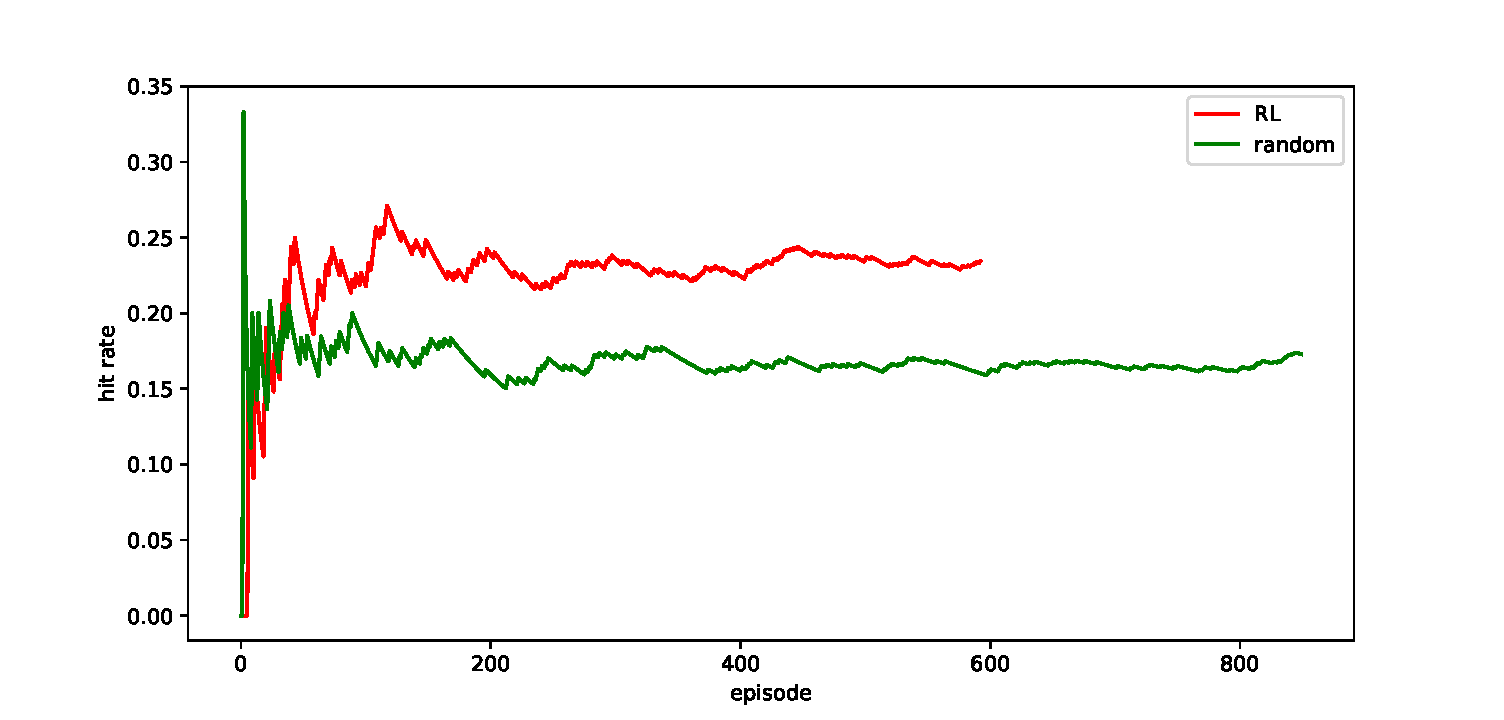
\includegraphics[width=0.8\linewidth]{figures/inv.pdf}
    }\hfill
    \subfloat[归纳不变式命中率]{
        \label{fig:ind}
        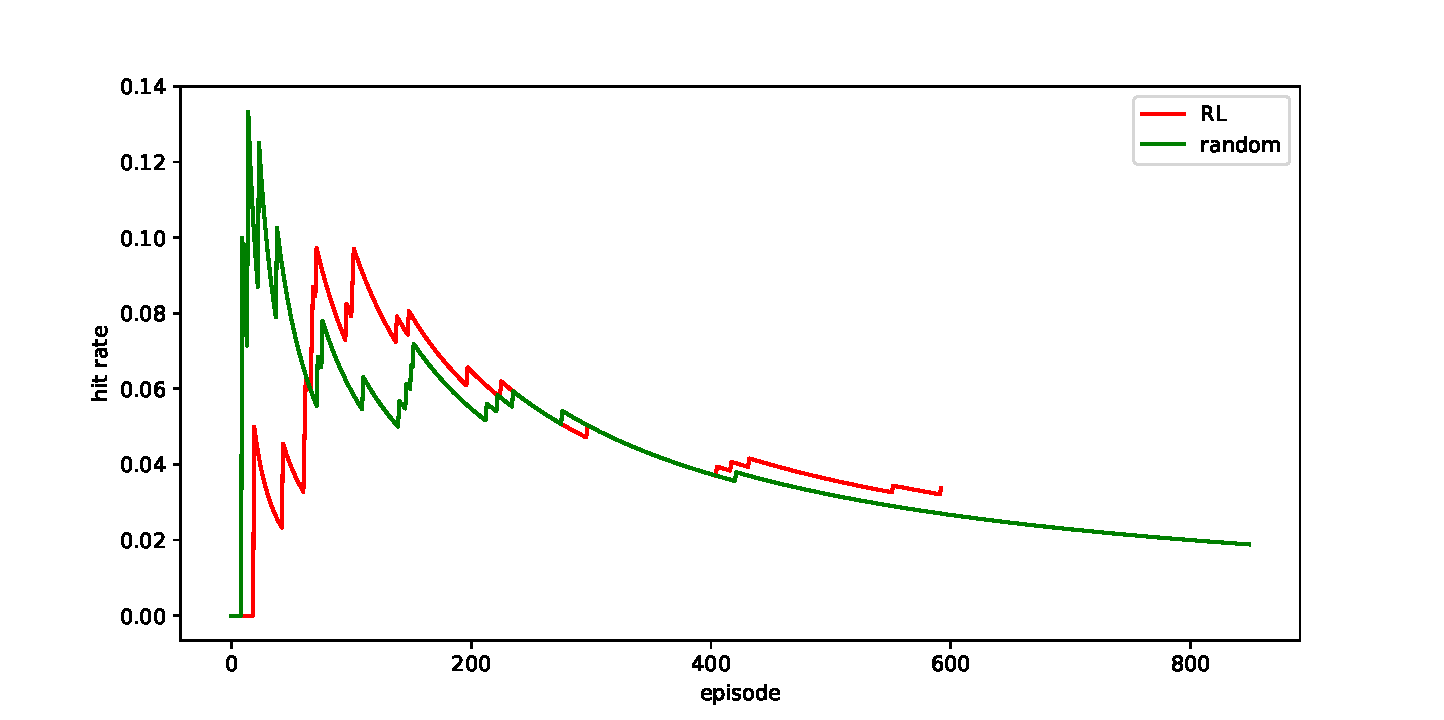
\includegraphics[width=0.8\linewidth]{figures/ind.pdf}
    }\hfill
    \caption{强化学习选择和随机选择的命中率}
    \label{fig:all}
\end{figure}
